\documentclass[18pt]{beamer}

\usepackage{graphicx}
\usepackage{titlesec}
\usepackage{listings} % For inserting code
\usepackage[margin=0.5in]{geometry} % For adjusting the margin size
\usepackage{wrapfig}
\usepackage{mathtools}
\usepackage{multicol}
\usepackage{array}
\usepackage{calc} % For wrapping lines in a table
\usepackage{tkz-kiviat} % For inserting a Kiviat (radar chart) diagram
\usepackage{adjustbox} % For formatting of Kiviat diagram
\usepackage{color} % So that we can have some dank colours on the kiviat diagram
\usetikzlibrary{arrows}

% For the bibliography
\setbeamertemplate{bibliography entry title}{}
\setbeamertemplate{bibliography entry location}{}
\setbeamertemplate{bibliography entry note}{}

\newcommand{\LegendBox}[3][]{%
\xdef\fitbox{}%
\coordinate[#1] (LegendBox_anchor) at (#2) ;
    \foreach \col/\item [count=\hi from 0] in {#3} {
       \node[color = \col,draw,
             fill  = \col!50,
             minimum width  = 4 ex,
             minimum height = 2 ex,
             label={[anchor = left,name=b\hi]right:\item}] at ([yshift=\hi*4 ex]LegendBox_anchor) {};
             \xdef\fitbox{\fitbox(b\hi)}
   }%
 \node [draw,fit=\fitbox(LegendBox_anchor)] {};
}

\newcolumntype{L}{>{\let\newline\\\arraybackslash}m{#1}} % For tidier tables


\usetheme{metropolis}           % Use metropolis theme
\title{G54SOD}
\subtitle{Developing a Smart Campus}
\date{Spring 2017}
\author{Richard Davies, Elias Khoury, Rub\'{e}n Escocia, Abdullah Masud}
\institute{The University of Nottingham}
\begin{document}
    \graphicspath{ {images/} }
    \maketitle

    \begin{frame}{Breakdown}
        \begin{enumerate}
            \item Initialisation
            \item Heuristic application
            \item Killing the weak
        \end{enumerate}
    \end{frame}


    \begin{frame}{The Problem}
        \begin{enumerate}
            \item Waste management on campus is a complex process \pause
            \item Sanitation workers need to tour the campus to empty bins \pause
            \item Campus is so large that bins are not always full \pause
            \item This wastes the time of sanitation workers \pause
            \item By using sensors we can detect which bins need emptying \pause
            \item Is this more efficient?
        \end{enumerate}
    \end{frame}

    \begin{frame}{Different Methods of Simulation}
        \begin{centering} 
            \begin{tabular}{| c | c | c |}
                \hline
                Agent Based      & Discrete Event  & System Dynamic \\
                \hline
                \pause
                Student Movement & Cafe Acoustics    & Online Car Pool \\ \pause
                                 & Parking Fullness  & Pre-order Student Lunch \\ \pause
                                 & Waste on Campus   & \\
        
                \hline

            \end{tabular}
        \end{centering}
    \end{frame}


    \begin{frame}{Introduction}
        \begin{columns}
            \column{0.5\textwidth}
                A smart campus is
                \begin{itemize}
                    \item Efficient
                    \item Safe
                    \item Sustainable
                    \item Responsive
                    \item Enjoyable Place to live and work
                    \item Underpinned and enhanced by digital or internet based technologies
                \end{itemize} \cite{Misc:uonsmartcampus}
            \column{0.5\textwidth}
                \begin{figure}
                
\includegraphics[width=0.99\columnwidth]{smart}
                \caption{Can we make Nottingham University smart?}
                \end{figure}
        \end{columns}
    \end{frame}

    \begin{frame}{Feasibility Measures}
        \begin{adjustbox}{max totalsize={.9\textwidth}{.7\textheight},center}
        \begin{tikzpicture}
          \tkzKiviatDiagram{Coolness, Cost, Feasibility, Acceptability, Demand, Practicality, Adaptation, Integration, Expansion}
          \tkzKiviatLine[thick,
                       color      = orange,
                       mark       = none,
                       mark size  = 4pt,
                       opacity    = .2,
                       fill       = orange!20,
                       opacity=.5](8,7,8,7,7,7,6,8,7)
          \tkzKiviatLine[thick,
                        color      = red,
                        mark       = none,
                        ball color = red,
                        mark size  = 4pt,
                        opacity    = .5,
                        fill=red!20](5,4,8,5,6,7,8,8,2)
          \tkzKiviatLine[thick,
                        color      = brown,
                        mark       = none,
                        mark size  = 4pt,
                        opacity    = .5,
                        fill       = brown!20,
                        opacity=.5](6,7,7,6,6,6,7,6,5)
          \tkzKiviatLine[thick,
                       color      = blue,
                       mark       = none,
                       mark size  = 4pt,
                       opacity    = .5,
                       fill       = blue!20,
                       opacity=.5](5,2,6,4,4,6,1,1,1)
          \tkzKiviatLine[thick,
                       color      = green,
                       mark       = none,
                       mark size  = 4pt,
                       opacity    = .5,
                       fill       = green!20,
                       opacity=.5](5,7,5,5,3,6,6,5,7)
          \tkzKiviatLine[thick,
                       color      = purple,
                       mark       = none,
                       mark size  = 4pt,
                       opacity    = .5,
                       fill       = purple!20,
                       opacity=.5](3,3,4,4,3,2,2,2,2)

            \LegendBox[shift={(1cm,-1cm)}]{current bounding box.south east}%
            {red/Remodel Layout of Cafe,
             blue/Cafe Acoustics,
             green/Carpooling,
             purple/Preordering Student Lunches,
             pink/Parking Simulation,
             orange/Automated Waste Management}
         \end{tikzpicture}
     \end{adjustbox}
    \end{frame}

    \begin{frame}{Stakeholder Views}
        \begin{center}
        \begin{tabular}{|p{0.3\textwidth} | p{0.3\textwidth} | p{0.3\textwidth}|}
            \hline
        	Students & University Personnel & System Designers \\
            \hline
        	Main driving force of the waste system & Employ the waste staff & Discuss feasibility of the system \\
            \hline
            Desire a clean campus & Comprised of the waste staff & Responsible for maintenance \\
            \hline
            & Own the campus & \\
            \hline
        \end{tabular}
        \end{center}
    \end{frame}


    \begin{frame}{Replacing or Relocating}
        \begin{columns}
            \column{0.5\textwidth}
            \begin{itemize}
                \item The workload for the cleaning staff would be reduced, therefore fewer people would be required
                \item This situation might be beneficial for the university due to all the money that would be saved
                \item On the other hand, many families would stop receiving an income and relocating the cleaning staff might be a more ethical solution
            \end{itemize}
            \column{0.5\textwidth}
            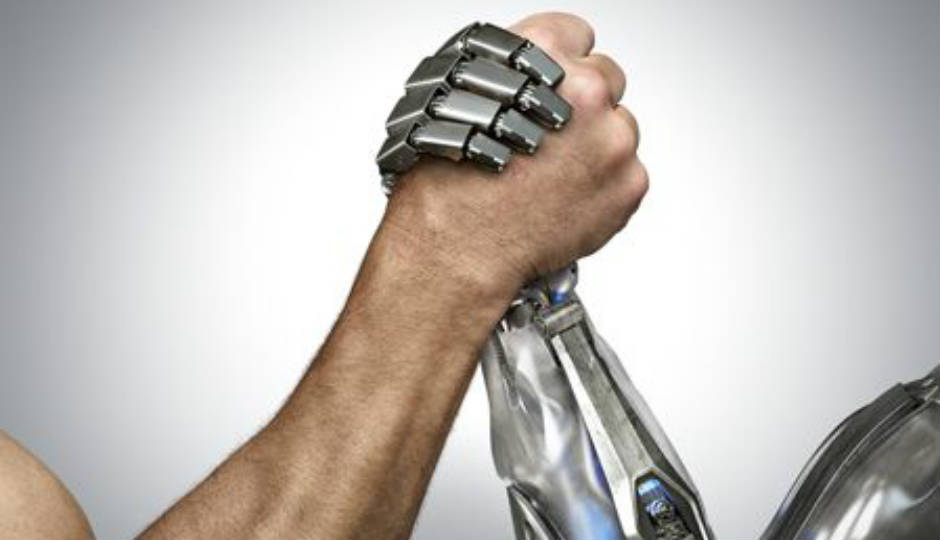
\includegraphics[width=0.99\columnwidth]{humanvsrobot}
        \end{columns}
    \end{frame}

    \begin{frame}{Student Opinions}
        \begin{columns}
            \column{0.5\textwidth}
            \begin{itemize}
                \item Less trash around the campus would improve its image
                \item Removing geese faeces would reduce the risk of potential diseases
                \item Students are less likely to litter on a cleaner campus
                \item A cleaner campus could lead to a better understanding of sustainability
            \end{itemize}
            \column{0.5\textwidth}
            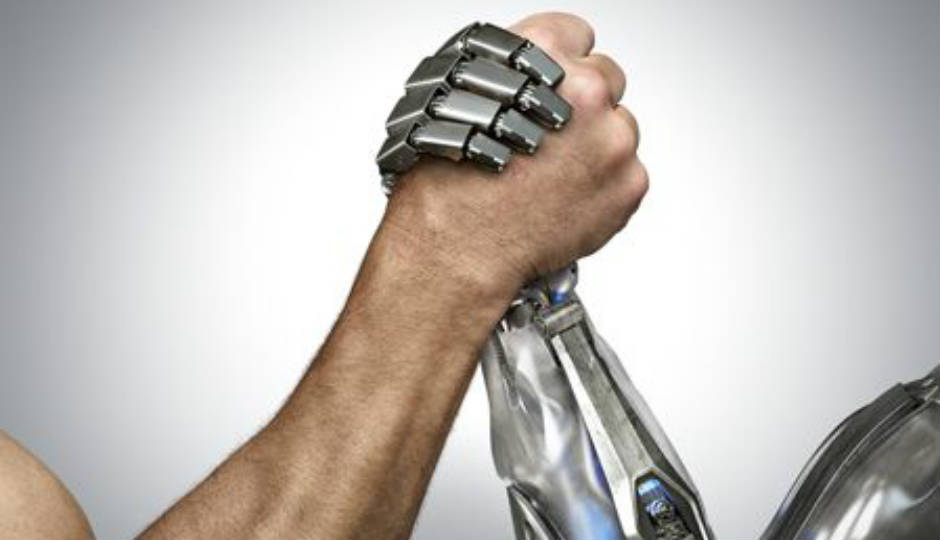
\includegraphics[width=0.99\columnwidth]{humanvsrobot}
        \end{columns}
    \end{frame}

    \begin{frame}{University Opinions}
        \begin{columns}
            \column{0.5\textwidth}
            \begin{itemize}
                \item The workload for the cleaning staff would be reduced, therefore fewer people would be required
                \item This situation might be beneficial for the university due to all the money that would be saved
                \item On the other hand, many families would stop receiving an income and relocating the cleaning staff might be a more ethical solution
            \end{itemize}
            \column{0.5\textwidth}
            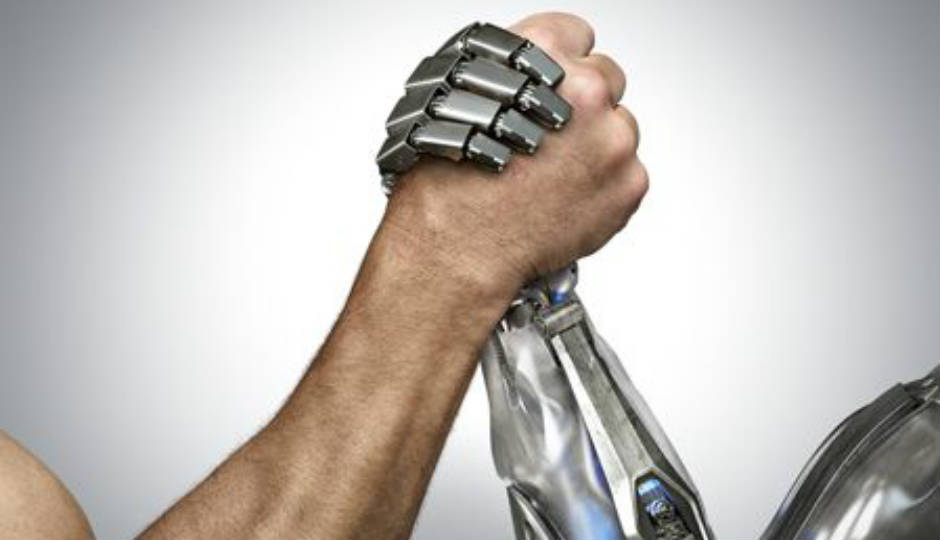
\includegraphics[width=0.99\columnwidth]{humanvsrobot}
        \end{columns}
    \end{frame}

    \begin{frame}{Replacing or Relocating}
        \begin{columns}
            \column{0.5\textwidth}
            \begin{itemize}
                \item The workload for the cleaning staff would be reduced, therefore fewer people would be required
                \item This situation might be beneficial for the university due to all the money that would be saved
                \item On the other hand, many families would stop receiving an income and relocating the cleaning staff might be a more ethical solution
            \end{itemize}
            \column{0.5\textwidth}
            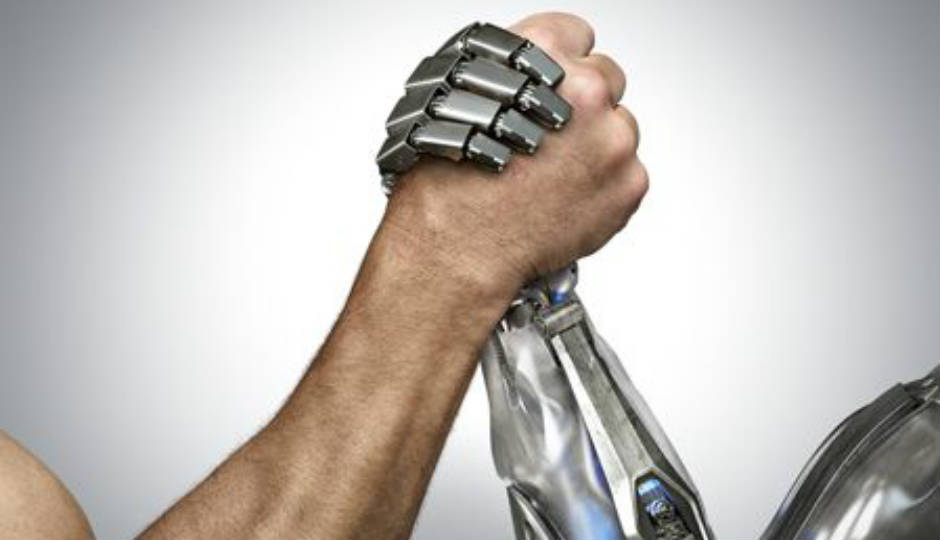
\includegraphics[width=0.99\columnwidth]{humanvsrobot}
        \end{columns}
    \end{frame}

    \begin{frame}{Selection}
        \begin{columns}
            \column{0.5\textwidth}
                \begin{figure}
                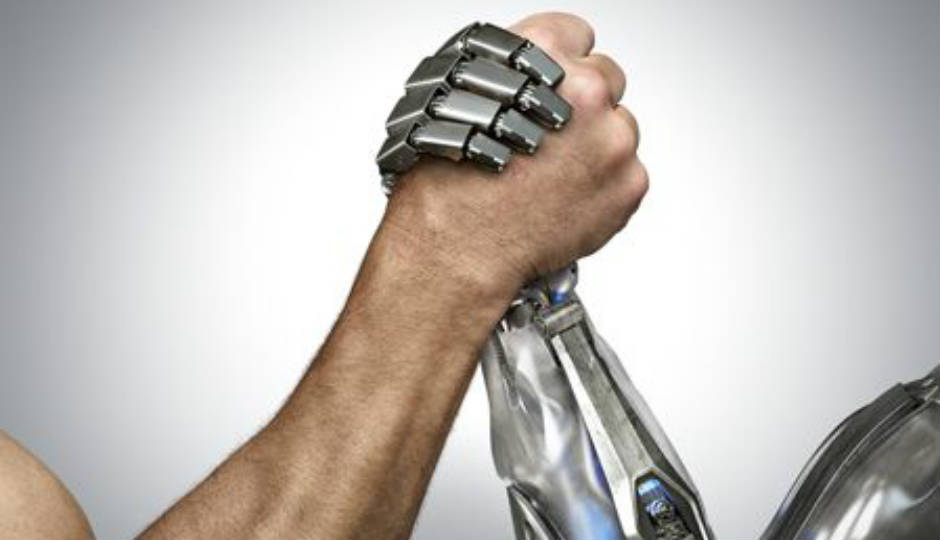
\includegraphics[scale=0.25]{humanvsrobot}
                \end{figure}
            \column{0.5\textwidth}
                Each chromosome gets a $ \frac{1}{n} $ chance\\
                But better ones get a bigger probability
        \end{columns}
    \end{frame}


    \begin{frame}{Proposed Project}
        \begin{itemize}
            \item Use sensors in the bins to detect when a bin is full \pause
            \item At night calculate the shortest route on campus. \pause
            \item Simulate different situations and compare with simply visiting each bin. \pause
                \begin{itemize}
                     \item Random bins full / Only one bin full / etc.\pause
                     \item Simulate over a week to see if not emptying bins leads to consequences the next day. \pause
                \end{itemize}
            \item Be ale to detect garbage on the floor and notify sanitation worker.
        
        \end{itemize}
    \end{frame}
    
    \begin{frame}[allowframebreaks]
            \frametitle{References}
            \bibliographystyle{plain}
            \bibliography{presentation}
    \end{frame}

\end{document}
